\documentclass[parskip=full]{scrartcl}
\usepackage[utf8]{inputenc} % use utf8 file encoding for TeX sources
\usepackage[T1]{fontenc}    % avoid garbled Unicode text in pdf
\usepackage[german, english]{babel}  % german hyphenation, quotes, etc
\usepackage{graphicx}       % provides commands for including figures
\usepackage{rotating}
\usepackage{amsmath}
\usepackage{pdfpages}
\graphicspath{ {images/} }
\usepackage{hyperref}       % detailed hyperlink/pdf configuration
\hypersetup{                % ‘texdoc hyperref‘ for options
pdftitle={PSE : LAMeetsML},%
bookmarks=true,%
}
\usepackage{csquotes}       % provides \enquote{} macro for "quotes"
\usepackage[nonumberlist, acronym]{glossaries} % provides glossary commands
\usepackage{enumitem}
\usepackage{lscape}
\usepackage{caption}
\usepackage{placeins}


\makenoidxglossaries
%
%%Glossary
%

\newglossaryentry{memento}
{
	name=Solver,
	plural=Solvers,
	description={In mathematics and computer science, an Solver is an unambiguous specification of how to solve a class of problems. Solvers can perform calculation, data processing and automated reasoning tasks}
}
\newglossaryentry{ginkgo}
{
	name=Solver,
	plural=Solvers,
	description={In mathematics and computer science, an Solver is an unambiguous specification of how to solve a class of problems. Solvers can perform calculation, data processing and automated reasoning tasks}
}



\begin{document}

\begin{titlepage}
\centering
{\scshape\LARGE Karlsruher Institut für Technologie\par}
\vspace{1cm}
{\scshape\Large Design Document\par}
\vspace{1.5cm}
{\huge\bfseries Numerical Linear Algebra meets Machine Learning \par}
\vspace {2cm}

{\Large\itshape Fabian Koffer\par}
{\Large\itshape Simon Hanselmann\par}
{\Large\itshape Yannick Funk\par}
{\Large\itshape Dennis Leon Gr\"{o}tzinger\par}
{\Large\itshape Anna Katharina Ricker\par}

\vfill
Supervisors\par
Hartwig Anzt
Makus G\"{o}tz

\vfill
{\large\today\par}
\end{titlepage}

\tableofcontents
\newpage


\section{Class descriptions}

\subsection{Collector}
\subsubsection{Class Collector}
The Collector class is responsible for collecting a given amount of matrices and saving it into a HDF5 dataset.
When the user types collect into the CLI, a collector Object will be created and the public method collect() with its parameters:

amount, name, size, density and path will be called. The class has a Saver class attribute and a Generator class attribute.

amount, name, size, density and path will be called. The class has a Saver class attribute and a Generator class attribute. 

It uses methods from the Generator class to get matrices to collect and methods from the Saver class to save the collected dataset.
(see the collect method Activity Diagram for a more detailed overview).
The Collector class is the interface between matrix collecting and the CLI and conceals all the classes of the Collector described in the following.

\subsubsection{Class Saver}

The Saver class is just responsible for saving a given matrix dataset.
Its only method is the save(dataset, name, path) method, which
is called by the collect method from an Collector object.

The Saver class is just responsible for saving a given matrix dataset. Its only method is the save(dataset, name, path) method, which
is called by the collect method from an Collector object. 

The save method takes an NPArray as a matrix dataset, converts it into an HDF5 file and saves it into a given directory with a given name.

\subsubsection{Class Generator}
The Generator class is responsible for actually generating matrices by transforming raw matrices from SuiteSparse and validating them.
The generate(size, density):Matrix method is called by a Collector object, uses the Matrix class to initialize an empty matrix, uses the Ssget class to fetch and transform matrices from the SuiteSparse collection and uses the static Validator.validate method to check if the matrix is regular and can be returned.

\subsubsection{Class Ssget}
The Ssget class is responsible for fetching matrices from the SuiteSparse collection, transforming them and returning them.
Its getMatrix method is called by a generator object.
The getMatrix method uses the Matrix class to initialize a matrix, then the private downloadMatrix method to fetch a matrix from SuiteSparse, and after that uses its private cutMatrix method to cut a fixed size, regular matrix out of it.

\subsubsection{Class Validator}

The Validator class is a util class and responsible for validating given matrices(checking for regularity)
 Its only static method validate takes a matrix and returns true for regular, and false for not regular.

\subsubsection{Class CommandLineInterface}
The view represents the concrete command line interface. 

The Validator class is a util class and responsible for validating given matrices(checking for regularity).
Its only static method validate takes a matrix and returns true for regular, and false for not regular.

\subsubsection{Class View}
The view represents the command line interface. 

Therefore it only consists of two methods. 
The first one is readInput that receives a message that will be displayed and reads the next user input. 
The other method is createOutput. 
This method prints a string to the CLI.


\subsubsection{Interface OutputService}
The OutputService interfaces can be implemented and passed to a module to receive the output of the modules. 
Therefore it has methods that represent different ways output can be displayed. 

\subsubsection{Class Controller} 
The controller is the main entry point for the program execution. 
It creates the view, receives the user input, calls the parser to create a command from the input and starts the module the user wants.


 \subsubsection{Interface Subscriber}
The Subscriber interface only provides the method update() which will be triggered by an Observable upon receiving new values.

\subsubsection{Class Observable} 

\subsubsection{Interface OutputService}
The OutputService interfaces can be implemented and passed to a module to receive the output of the modules. 
Therefore it has methods that represent different ways output can be displayed. 

 \subsection{Interface Subscriber}
The Subscriber interface only provides the method update() which will be triggered by an Observable upon receiving new values.

\subsection{Class Observable} 

The Observable class can be used to notify Subscribers when new values are provided.
Subscribers can subscribe themselves to an Observer to be notified get notifications.
The next() method calls update() on each subscriber.


\subsection{Class CLIOutputService}
This class implements the OutputService and the Subscriber interface. 
On creation it gets a reference of the View to which it will pass the lines the modules wants to output.
It also implements the Subscriber interface to subscribe itself to an observable.
This can be used to display lines that are overwritten with new values like an progress bar or a counter.

\subsection{Class ClIOutputService}
This class implements the OutputService and the Subscriber interface. 
On creation it gets a reference of the View to which it will pass the lines the modules want to output.
It also implements the Subscriber interface to subscribe itself to an observable.
This can be used to display lines that are overwritten with new values like an progress bar or counter.


\subsubsection{Class CommandParser}
The CommandParser is a class that only has one static public method.
This method receives the user input string and returns a command.

\subsubsection{Class Command}
The Command class holds all the information entered by the user that is needed to execute a module.
There is one command subclass for each module and the command class also validates that all parameters are available to run the module.
The command also has a execute method which runs the specific module with all the arguments it needs.

\subsection{Labeling Module}
The labeling module is responsible for the labeling of the sparse matrices. The label of a matrix describes which which preconditioner/iterative Solver combination solves the given matrix the fastest. The label is represented by a vector. Each entry in the vector corresponds to one preconditioner/iterative Solver combination. The entry of the fastest one is 1, all other entries are zero. The matrices with the corresponding labels will be used to train the neural network in the training module. 
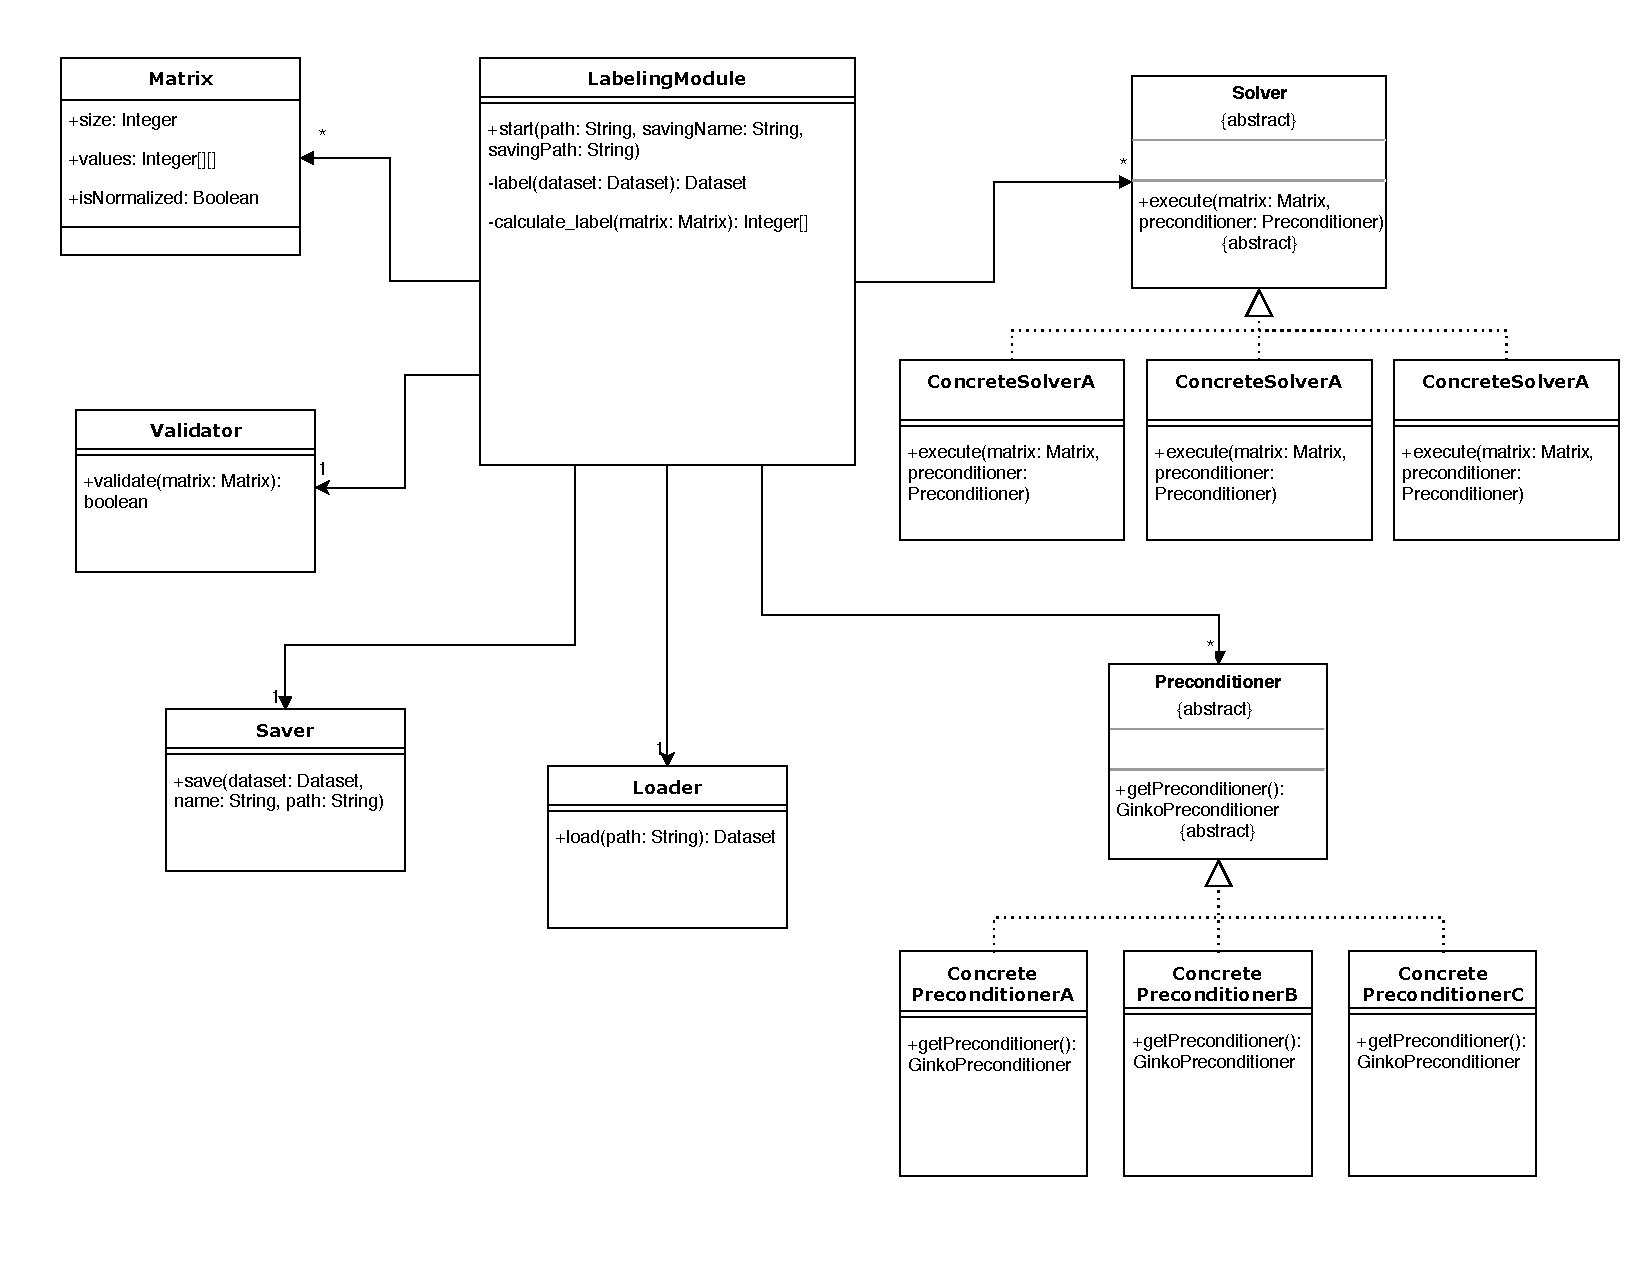
\includepdf{ClassDiagrams/PDF/LabelingModule_classdiagramm.pdf}
The main component of the labeling module is the class labeling module. It provides the only public method in the labling module, the method start(path:String, savingName:String,savingPath:String). This method is the entry point of the module and will start the labeling process of the provided matrices(specified by the path). \newline\newline

The class labeling modue has a set of matrices which the module will label.\newline\newline

The module furthermore has a Loader class. The class labeling module has exactly one Loader class. This class is responsible for loading the matrices which get labeled. Its only method is the method load(path:String) which gets a path of a hdf5 file supplied and returns a dataset. If the specified path is not a hdf5 file, the programm will print an error to the command line. \newline\newline

Another class in the labeling module is the Saver class. The class labeling module has exactly one Saver class. This class is responsible for the saving of the matrices and the labels. Its only method is the method save(dataset:Dataset,path:String). If this method is called, the specified dataset will be safed at the specified path. The matrices and the labels will be safed in one hdf5 file.\newline
\newline

Since the labeling module is responsible for finding the best preconditioner/iterative Solver combination for a given set of matrices, the module furthermore has a preconditioner and a Solver class. Those classes are abstract. ConcreteSolvers inherit from the class Solver and ConcretePreconditioners from the class Preconditioner.\newline\newline

The Solver class contains the logic for solving a matrix with an iterative Solver. Each ConcreteSolver corresponds to one iterative Solver.Each class of ConcreteSolver has the method execute(Matrix,Preconditioner) which will solve a given matrix. We will be using the design pattern "stragety" for the iterative Solvers. The reason being that each Solver does basically the same thing(solving a matrix) in a different manner. The user moreover has no influence on which Solver we will be using at any given time. 
Each Solver will take an optional precondtioner as its input for the method execute(Matrix,Preconditioner). The preconditioner will be used at every step of the iterative Solver. We will be using the design pattern "strategy" for the Preconditioners too. Preconditioners each return a GinkoPreconditioner which will be used by the Solver class to communicate with the ginkgo libary. So each ConcretePreconditioner basically does the same thing(returning a preconditioner). The user furthermore has no influence on which preconditioner we will be using at any given time. That is why the "strategy" design pattern is applicable

\subsubsection{Class LabelingModule}
activity diagram
\subsubsection{Class Solver}
An Solver in our sense is an interative Solver which is able to to solve a linear system Ax=b for x, where A is a (in our case sparse) matrix of size nxn, x is a vector of size 1xn and b is vector of size 1xn(n$\in$N).
%find correct symbol for N
The iterative Solver uses an iterative approach to solve the matrix. An iterative approach is characterized by the idea that the matrix gets solved step by step, where the solution of one step enables the solution of the next step. The class iterative Solver achieves this by communicating with the ginkgo libary, which has an implementation of the solvers. An iterative Solver may optionally use a preconditioner for its calculation. Since there are many different iterative Solvers which achieve the same outcome(solving for x) we will be using the design pattern "strategy". That is why the class Algortihm is abstract and ConcreteSolvers (which actually represent one iterative Solver each) will inherit from Solver. The user at no point decides which Solver gets used at any given time. \newline
An Solver one has one method execute(Matrix,Preconditioner) ,which takes a matrix (and a preconditioner) and solves it. The time the iterative Solver takes to solve the matrix will be recorded and in the class labelingModule used to label the matrix. All ConcreteSolvers have to implement the abstract function execute.

\subsubsection{Class ConcreteSolver}
A ConcreteSolver is the actual representation of one iterative Solver. 
\subsubsection{Class Preconditioner}
A preconditioner is a transformation of a linear system Ax=b for x, where A is a (in our case sparse) matrix of size nxn, x is a vector of size 1xn and b is vector of size 1xn(n$\in$N). A transformation may be a Matrix p (nxn) which would result in the linear system PAx = Pb. A preconditioner is used so that the linear system may be solved more easily by an iterative Solver. The transformation of the preconditioner is applied in every step of an iterative Solver. \newline\newline
The class Preconditioner only has one method, getPreconditioner() which will return the GinkoPreconditioner corresponding to the preconditioner class. The preconditioner class achieves this by communicating with the ginkgo libary. 
\subsubsection{Class ConcretePreconditioner}
A ConcretePreconditioner is the actual representation of one preconditioner.

\subsection{Training module}
The training module is responsible for the training and testing of a neural network. It is structured in 2 parts, the configuration file and the class training module. The class training module loads its configuration in the configuartion file. It furthermore uses a set of labled matrices for the training and testing. With the configuration set, the class training module will start the training and testing. The trained network will be saved to a specified path.
%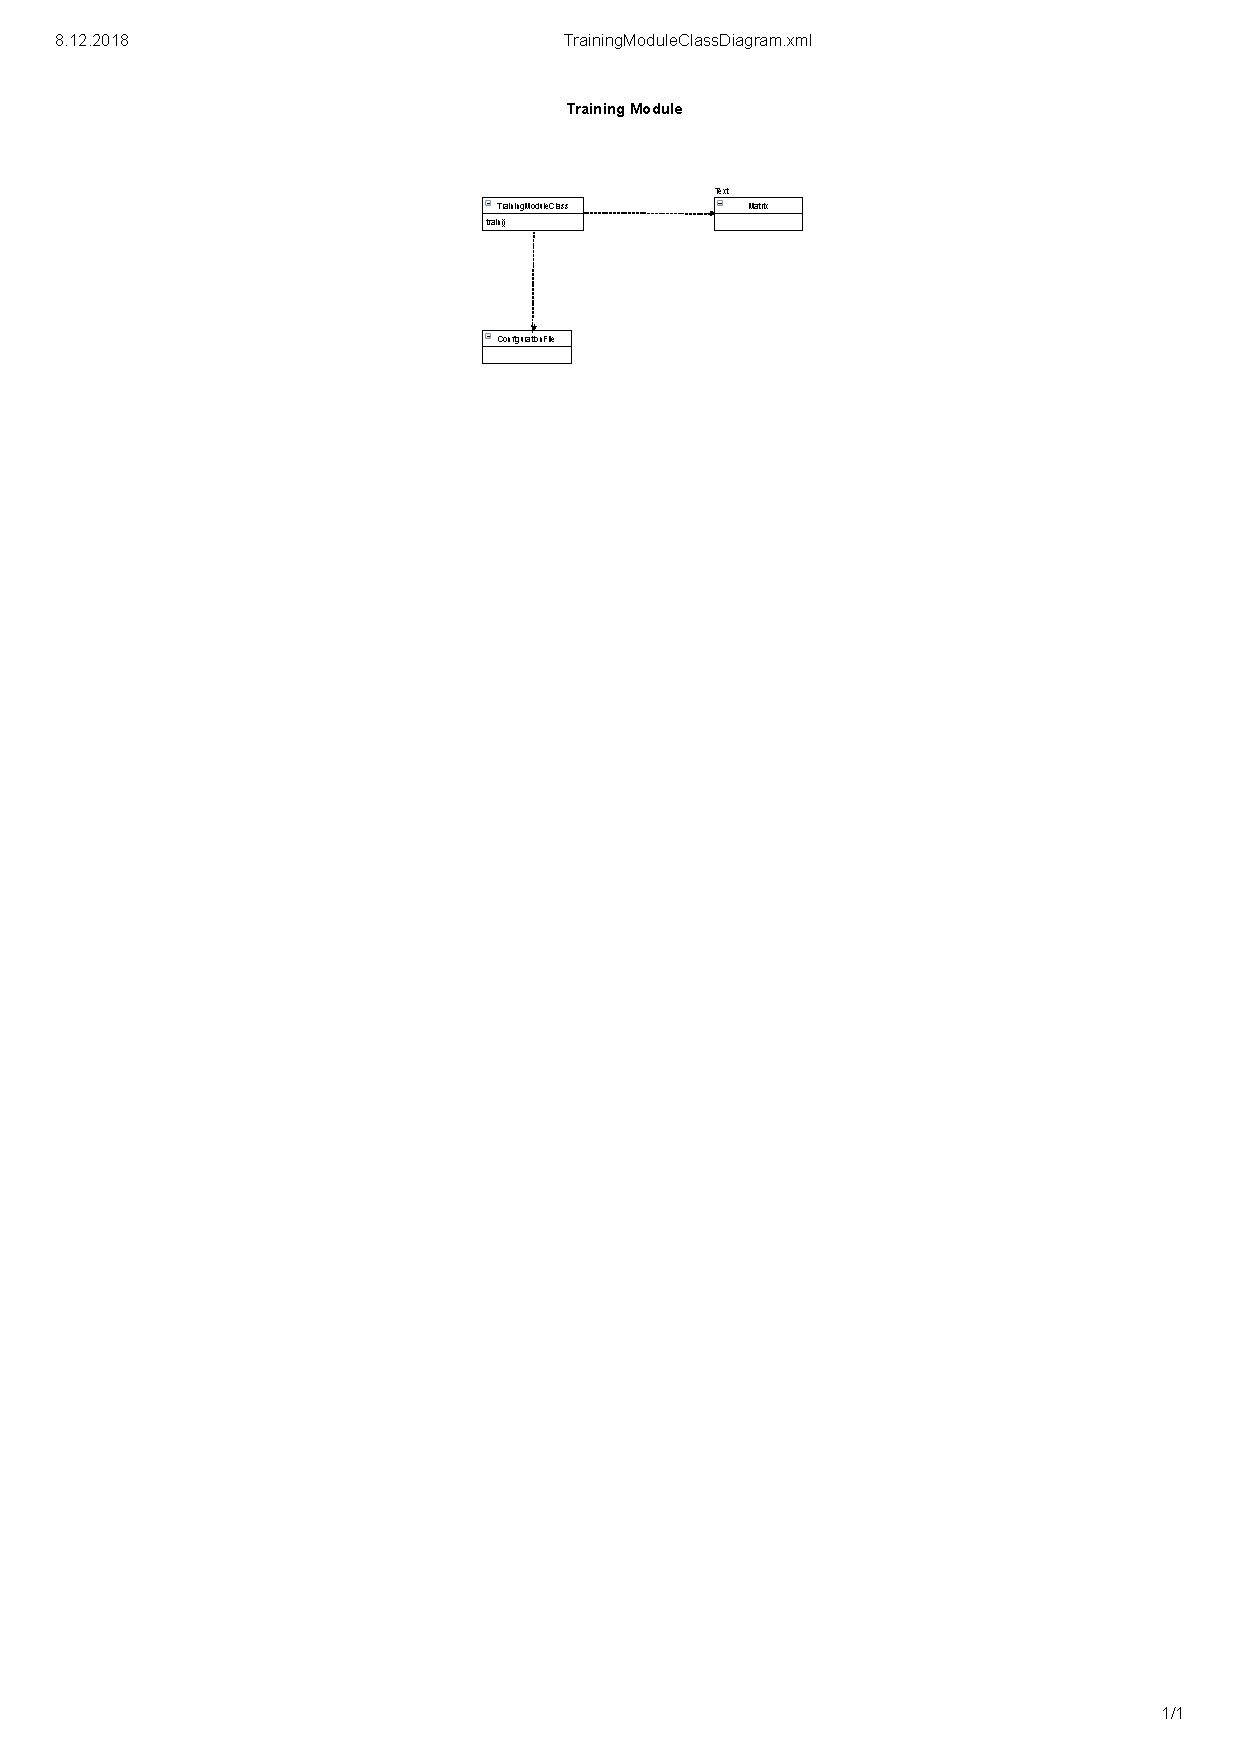
\includepdf[pages={1}]{ClassDiagrams/PDF/TrainingModuleClassDiagram}
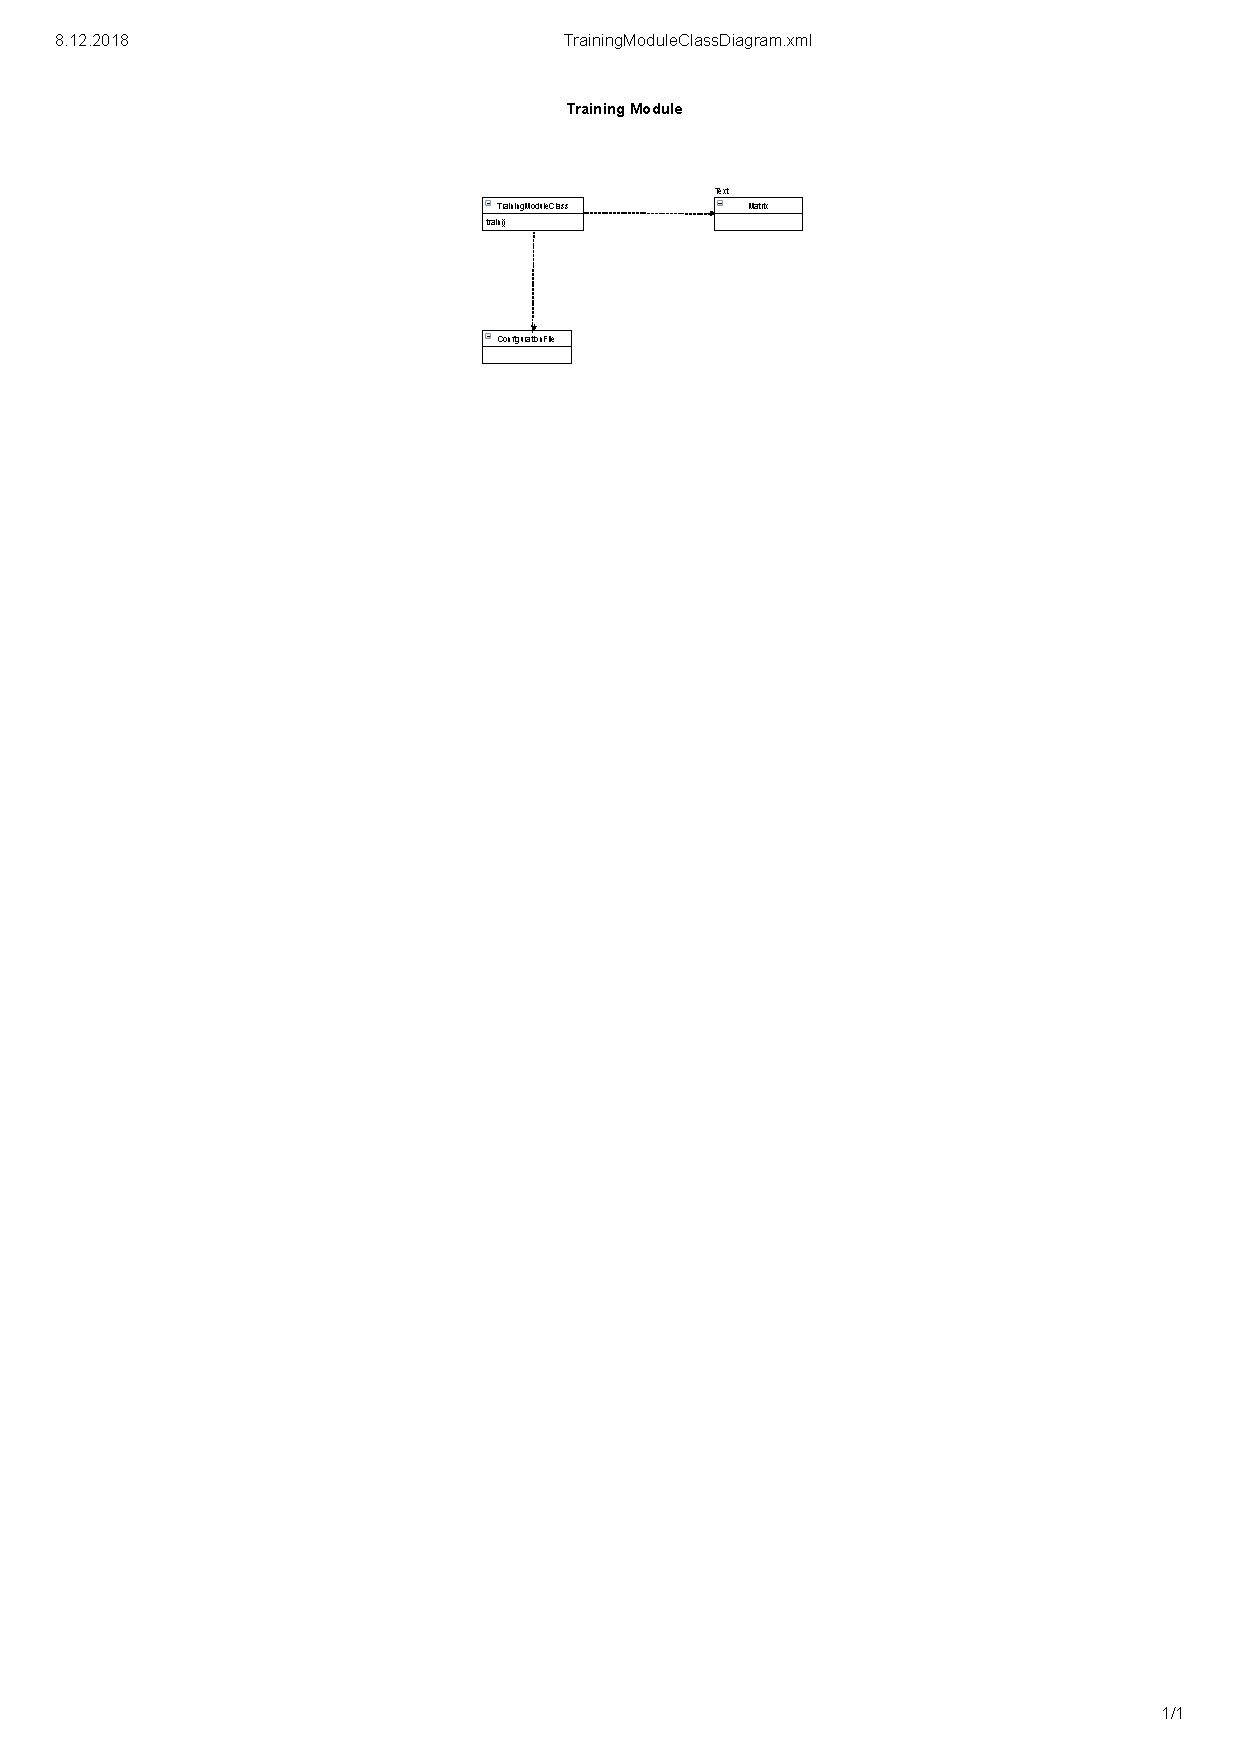
\includegraphics{ClassDiagrams/PDF/TrainingModuleClassDiagram.pdf}

\subsubsection{Class Configuration File}
The configuration file is a text file.
It is used to specify all necessary information the class neural network needs to train the neural network.
If the user does not change anything in the configuration file, defaut options will be used.The configuration file is organized in four main categories. 
\begin{enumerate}
\item loading path of the set of matrices 
\item saving path for the neural network
\item loading path for the neural network
\item model definition and hyperparameters  
\end{enumerate}
The loading path of the set of matrices is the path in which the matrices that are used for the training and testing are stored.
The training module only supports one hdf5 file.
If the path is any other file, the labling module will print an error(would crashing make sense if the user has to change the config file anyway?).
For the training and testing making sense there should be at least 500 matrices in the hdf5 file.
Otherwise the accuracy of the neural network will be so low that i can not be used for classification.
If there is no path specified, the training module will use a default path.
In the default path will be the latest matrices that the labling module has produced. \newline

The saving path for the neural network is the path where the trained and tested neural network will be safed.
It will be safed as a Keras model.
If there is no path specified, the neural network will be safed at a default destination.
If there is no path for the neural network specified in the module Classifier the module will use this default path to load its neural network.\newline

The loading path for the neural network is strictly optional.
If this path is specified the training module will use the neural network in the path for training and testing.
This option enables the user to use a pre-trained neural network for training.
This could be the case if the user interrupts the training process at a certain time and wants to to repeat the training later.
Other use cases are of course possible too.
The neural network has to be a model of the Keras framework. If the path is any other file the training module will print an error(crash?).
If this path is not specified the training module will create a new neural network(with the model definition and hyperparamters of the next category) and train with it. \newline

The model definition and hyperparameters are used to determine which neural network will be trained and tested. The model definition determines the following:
\begin{itemize}
\item the amount of layers
\item the amount of nodes in every layer
\item the kind of neural network(e.g. Convolutional)
\item the activation function
\item the regularization
\end{itemize}

The hyperparamters determine the following:

\begin{itemize}
\item the dropout
\item the batch size
\item how much of the data should be training and how much should be testing data
\end{itemize}

\subsubsection{Class TrainingModule}
The TrainingModule class is responsible for the training and testing of a neural network.
It can not be instantiated, since it is a utility class.The structure is mainly oriented towards the keras workflow and will be further described later.
The class offers one public method, the method train(). \newline
When the user types train() in the CLI the method train in the class TrainingModule will be executed in the following manner(see the activity diagram for a graphical overview).
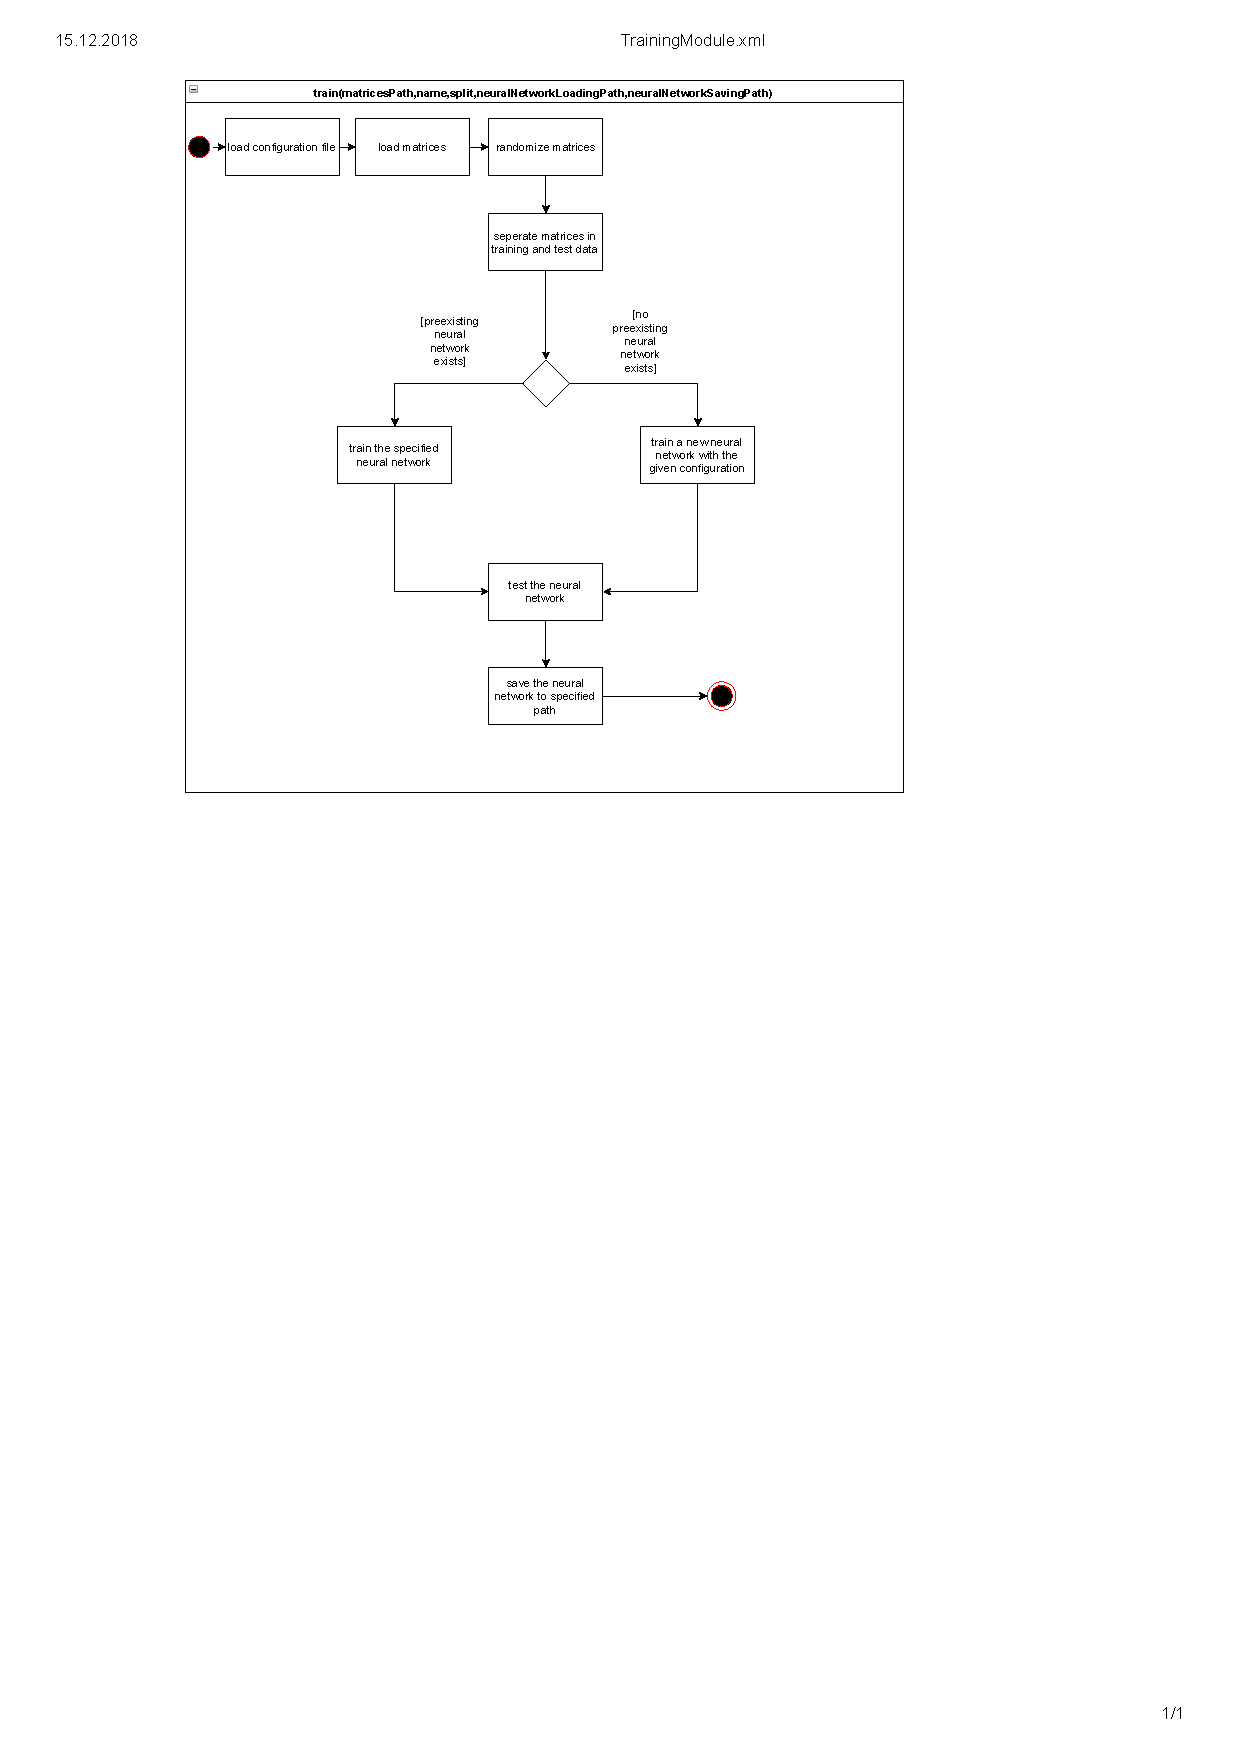
\includepdf[pages={1}]{ActivityDiagrams/PDF/TrainingModule}
\begin{itemize}
\item load the configuration file
\item load the matrices
\item seperate matrices in training and test data
\item train a preexisting neural network or a new one(depending on the configuration file)
\item test the neural network
\item save the neural network
\end{itemize}

The configuration file that gets loaded will be used to specify the subsequent points.\newline

The configuration file will determine from which path the labeled matrices will be loaded.
If there were no changes made in the configuration file, the default path will be used(see the class description of the configuration file).
The labeled matrices will be loaded in one hd5 file. If the path links to any other file, the class TrainingModule will print an error to the command line (crash?). \newline

After that the class TrainingModule will seperate the training and test data.
How the data will be seperated is specified in the configuration file.\newline

Following there are two alternatives
 If the user has specified a neural network in the configuration file, the class TrainingModule will train this neural network with the labeled matrices for the training.
If the user has not specified a neural network in the configuration file, the class TrainingModule will create a new neural network with the specifications in the configuration file.
If there are no model definitions in the configuration file the class TrainingModule will use the default neural network(see default neural network).
The class TrainingModule then proceeds with training the new neural network with the labeled matrices for the training. In both cases the current loss will be continously printed to the command line.\newline

Now the neural network is trained. The class TrainingModule proceeds with testing the neural network with the labeled matrices for the testing.
This process will determine the accuracy of the neural network on the given test matrices.
The accuracy will be printed on the command line.\newline

After that the neural network will be safed as a keras model.
The path for the saving is specified in the configuration file.

We will furthermore be using the function keras.callbacks.ModelCheckpoint to save the neural network after every epoch. This will guarantee that we do not loose all training progress if the computer crashes or other unexpected events happen. The proceedure is consitent with the design pattern "memento". 




\subsection{Classifier}
\subsubsection{Class Classifier}
\subsubsection{Interface Solver}
This interface is for the different Solvers for solving a given matrix.
\subsubsection{Class ConcreteSolver}
The Concrete Solver class is for solving a matrix in a certain way.
This means a certain approach to solve a matrix.
\subsubsection{Class Matrix}
\subsection{Classes which more than one Module uses}
\subsubsection{Class Loader}

\subsubsection{Class Validator}

\subsubsection{Class Neural Network}

\subsubsection{Class PatternImageCreator}
This class creates a Grayscale Sparcity Pattern Image out of a given matrix.
\subsubsection{Class GrayscaleSparcityPatternImage}


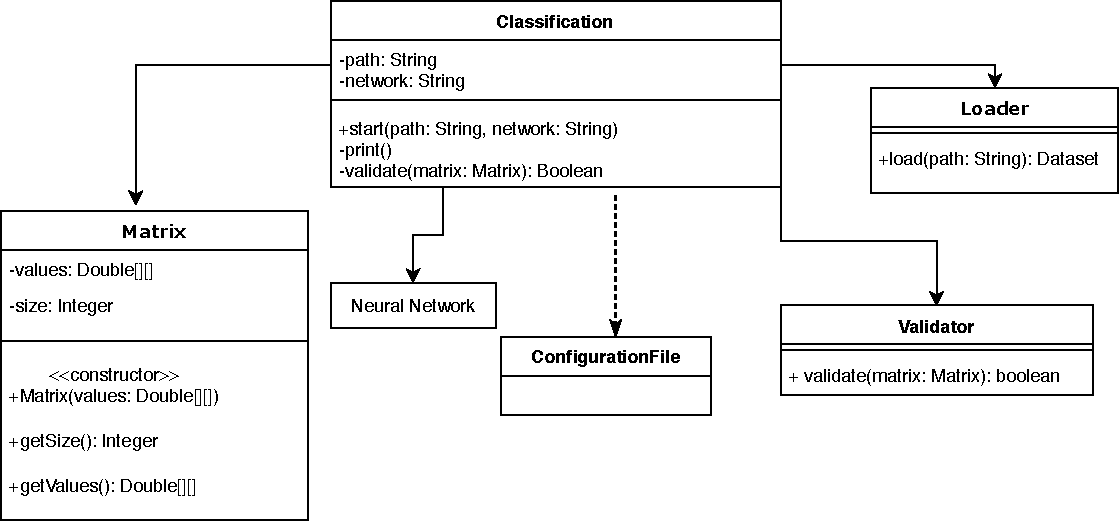
\includepdf[pages={1}]{ClassDiagrams/PDF/Classifier}

\section{Explanations}
\subsection{default neural network}
how is the nn structured(layers,activation function), what is it trying to achieve,...


\section{Sequence diagrams}

\section{Glossary}
%\glspl{collector}, labeling modle, neural network, classifier, default settings  \glspl{Dateiformat}

% % Automatisch generiertes Glossar (Latex zwei mal ausführen um Glossar anzuzeigen)
%
%\glsaddall % das sorgt dafür, dass alles Glossareinträge gedruckt werden, nicht nur die verwendeten. Das sollte nicht nötig sein!
\printnoidxglossaries

\end{document}
